\section{Lecture 5 (September 16th)}
\begin{recall}
Last time, we have dealt with $K[x]/(p(t))$ and minimal polynomials. Today, we will learn about properties of finite and algebraic extensions.
\end{recall}
\vspace{2ex}
\begin{defi}
(Simple field extensions) A field extension $F/K$ is simple if $F=K(\alpha )$ for some $\alpha \in F$, where $K(\alpha )$ denotes the smallest subfield of $F$ containing $K\cup \{\alpha \}$. Notice that the field extension is constructed from simply adding a single element. 
\end{defi}
\vspace{2ex}
\begin{rmk}
(Notation) $K(\alpha )$ is the smallest subfield, and $K[\alpha ]$ is the smallest subring of $F$ containing $K\cup \{\alpha \}$. Notice that these are equivalent to the definitions introduced last class due to inclusiveness and minimality.
\end{rmk}
\vspace{2ex}
\begin{rmk}
\begin{itemize}
\item[(i)] $\alpha \in F$ is algebraic over $K$ if and only if
\[\mathrm{ker}\Big(\mathrm{ev}_{\alpha }:K[t]\rightarrow F:f(t)\mapsto f(\alpha )\Big)\] 
is nontrivial.
\item[(ii)] If $\alpha $ is algebraic over $K$, then $K[\alpha ]=K(\alpha )$. In particular, every element of $K(\alpha )$ can be expressed as a polynomial in $\alpha $ with coefficient in $K$.	
\end{itemize}
\end{rmk}
\vspace{2ex}
\begin{proof}
Consider $\alpha \in F$. 
\[\mathrm{ker}(\mathrm{ev}_{\alpha })=(p(t))\]
and due to the first isomorphic theorem,
\[K[t]/(p(t))\cong K[\alpha ]\]
If $\alpha $ is algebraic over $K$, then $(p(t))$ must be a maximal ideal of $K[t]$. This implies that $K[\alpha ]=K(\alpha )$.
\end{proof}
\vspace{2ex}
\begin{prop}
Let $K\subset K(\alpha )=F$ be a simple extension. Then either
\begin{itemize}
\item[(i)] $F\cong K[t]/(p(t))$ for an irreducible monic polynomial $p(t)\in K[t]$ such that $p(\alpha )=0$
\item[(ii)] $F\cong K(t)$, the field of fractions of $K[t]$
\end{itemize}
In the first case, $[F:K]=\mathrm{deg}(p(t))$. In the second case, $[F:K]=\infty $. 
\end{prop}
\vspace{2ex}
\begin{ex}
(13.21) One example of a simple extension is
\[\alpha =2^{1/5}\in {\bm Q}(2^{1/5})\]
Notice that $\pi $ is algebraic in ${\bm R}$ but is not algebraic in ${\bm Q}$. 
\end{ex}
\vspace{2ex}
\begin{thm}
(7.11) Let $K$ be a field and $f(x)$ be a nonzero polynomial of degree $n$. Then,
\[K[x]/(f(x))\]
is a $n$-dimensional vector space over $K$.
\end{thm}
\vspace{2ex}
\begin{proof}
Notice that the following set is a basis for $K[x]/(f(x))$
\[\{1,x,\ldots ,x^{n-1} \}\]
\end{proof}
\vspace{2ex}
\begin{rmk}
(Notation) The minimal polynomial of $\alpha $ over $K$ is denoted $\mathrm{irr}(\alpha ,K)$.
\end{rmk}
\vspace{2ex}
\section{13.4 Algebraic Extensions}
\begin{defi}
(13.30) A field extension $F/K$ is algebraic if every element of $F$ is algebraic over $K$. 
\end{defi}
\vspace{2ex}
\begin{prop}
(13.31) Every finite extension $F/K$ is algebraic.
\end{prop}
\vspace{2ex}
\begin{proof}
Fix an element $\alpha \in F$. Set $\mathrm{dim}_{K}\,F=n$. Then
\[\{1,\alpha ,\alpha ^2,\ldots ,\alpha ^{n}\}\]
is linearly dependent over $K$, that is, $a_0+a_1\alpha +\ldots +a_{n}\alpha ^{n}=0$ for some $(a_0,\ldots ,a_{n})\ne {\bf 0}\in K^{n+1}$. Take
\[f(t)=a_0+a_1t+\ldots +a_{n}t^{n}\]
in $K[t]$ and it is a polynomial with coefficients in $K$ such that $f(\alpha )=0$.
\end{proof}
\vspace{2ex}
\begin{prop}
(13.13) Let $K\subset E\subset F$ be field extensions. If $E/K$ and $F/E$ are both finite, then $F/K$ is also finite. Furthermore, 
\[[F:K]=[F:E][E:K]\]
\end{prop}
\vspace{2ex}
\begin{proof}
Let $\{f_{i}\}^{n}_{i=1}$ be an $E$-basis of $F$ and $\{e_{j}\}^{n}_{j=1}$ be a $K$-basis of $E$. Then $\{f_{i}e_{j}\}$ is a $K$-basis of $F$. The rest is for you!
\end{proof}
\vspace{2ex}
\begin{rmk}
If $\alpha \in F$ is algebraic over $K$, then $K(\alpha )/K$ is finite, hence algebraic. This is because 
\[\mathrm{dim}_{K}\,K(\alpha )= \mathrm{deg}\Big(\mathrm{irr}(\alpha ,K)\Big)\]
Here,
\[\mathrm{dim}_{K}K(\alpha )=\mathrm{dim}_{K}K[t]/(\mathrm{irr}(\alpha ,K))\]
as
\[K[t]/(\mathrm{irr}(\alpha ,K))\cong K[\alpha ]=K(\alpha )\]
due to the 3rd isomorphism theorem.
\end{rmk}
\vspace{2ex}
\begin{prop}
A field extension $F\,/\,K$ is finite if and only if there are algebraic elements $\alpha_1,\alpha_2,\ldots,\alpha_{r}$ over $K$ such that $F=K(\alpha_1,\alpha_2,\ldots ,\alpha_{r})$.
\begin{center}
\begin{tikzpicture}[baseline=(current bounding box.center)]
  \node (F) at (0,4) {$F$};
  \node (K) at (0,0) {$K$};
  \node (L) at (2,2) {$K(\alpha_1,\alpha_2,\ldots,\alpha_n)$};

  \draw (F) -- (K);
  \draw (F) -- (L);
  \draw (K) -- (L);
\end{tikzpicture}
\end{center}
\end{prop}
\vspace{2ex}
\begin{proof}
(if) Suppose we are given algebraic elements $\alpha_1,\ldots ,\alpha _{r}$ over $K$ such that $F=K(\alpha_1,\ldots ,\alpha_{r})$. Consider the tower of finite towers
\begin{center}
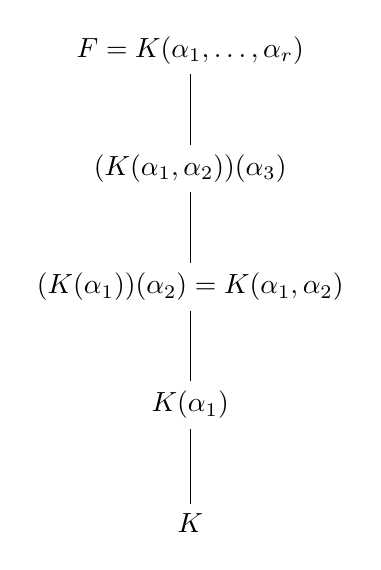
\begin{tikzpicture}[baseline=(current bounding box.center)]
  \node (F) at (0,1.5) {$F=K(\alpha_1,\ldots ,\alpha _{r})$};
  \node (G) at (0,0)   {$(K(\alpha_1,\alpha_2))(\alpha_3)$};
  \node (H) at (0,-1.5) {$(K(\alpha_1))(\alpha_2)=K(\alpha_1,\alpha_2)$};
  \node (I) at (0,-3) {$K(\alpha_1)$};
  \node (J) at (0,-4.5) {$K$};


  % lines (like the chalk sketch)
  \draw (F) -- (G);
  \draw (G) -- (H);
  \draw (H) -- (I);
  \draw (I) -- (J);
\end{tikzpicture}
\end{center}

\end{proof}
\vspace{2ex}

